% based on scrbook
% finaler Ablauf: übersetzen, Tools -> Benutzer -> MakeNomenclature, übersetzen
\documentclass[
fontsize=11pt, %font size
%paper=a4, %paper format
headsepline, %separating line for header
chapterprefix, % produce "Chapter ..."
numbers=noenddot, % no full-stop after last number
listof=totoc, %Entry in table of contents for list of figures/tables
index=totoc, %Entry in table of contents for index
bibliography=totoc, %Entry in table of contents for bibliography
%BCOR=5mm,%Binding correction, ensures sufficient space for binding
%todo change this to final to switch off for expamle the showlabels
%todo manually put 'disable' in front of usepackage{todonotes}
%final,%
]%
{scrbook}%


\KOMAoptions{twoside=false}

%% adjust spacing of chapters (start on top for working)
%\renewcommand*{\chapterheadstartvskip}{\vspace*{0cm}}
%\renewcommand*{\chapterheadendvskip}{\vspace{0cm}}






\usepackage{geometry}
\geometry{
a4paper,
total={150mm,205mm},
left=15mm,
right=50mm,
}

% 

% --------- Packages ----------
%\NeedsTeXFormat{LaTeX2e}
%\usepackage[dvips]{epsfig}
%\usepackage[latin1]{inputenc}
% TODO Argument "english" checken
\usepackage[english]{babel} 
%\usepackage[ngerman]{babel} 
\usepackage{a4wide}
%\usepackage{psfig}
\usepackage{fancyhdr}
\usepackage{latexsym}
\usepackage{enumerate}
\usepackage{paralist}
\usepackage{float}
\usepackage{verbatim}  % verbatiminput
\usepackage{caption}
\usepackage{floatflt}
\usepackage{afterpage}
\usepackage{graphicx}
\usepackage[space]{grffile}  % handles space in file name
\usepackage{moreverb}     
%\usepackage[]{mcode}
\usepackage{bbm}

% spacing of items: noitemsep 
\usepackage{enumitem}


% \usepackage{tabulary} % to set dith to side width and use left/right alignment
%\usepackage{showframe} % show margin of page


\usepackage[intoc]{nomencl}
\makenomenclature

% math
\usepackage{mathtools} % successor of \usepackage{amsmath}
\usepackage{amssymb,amsfonts}
\setcounter{MaxMatrixCols}{10} % leftover from Marcos
\usepackage{cases}

% Pseudo Code
\usepackage{algorithm}
\usepackage[noend]{algpseudocode}

%% bibliography
%%\usepackage[style=authoryear, backend=biber]{biblatex}
%%%\usepackage{biblatex}
%%\bibliography{bib}
%\usepackage[round, sort, comma]{natbib}
%\bibliographystyle{apalike}


% fraction for floats
\renewcommand{\floatpagefraction}{0.8}
%\renewcommand{\textfraction}{0.15}


% prevent floats from floating too much around (stay in one section)
%\usepackage[section]{placeins}

% adjust font of abbreviations
\usepackage{helvet}
\renewcommand{\nomlabel}[1]{{\fontfamily{phv}\selectfont \textbf{#1}}} %bold Helvetica



% ---------------------------------------------------------------------------------------------
% OWN PACKAGES 
% ---------------------------------------------------------------------------------------------

% tables
\usepackage{booktabs}
\usepackage{longtable}
\usepackage{tabularx} % especially for the title page
\newcolumntype{L}{>{\raggedright\arraybackslash}X}
\newcolumntype{Y}{>{\centering\arraybackslash}X}
\newcolumntype{R}{>{\raggedleft\arraybackslash}X}
\newcolumntype{x}{>{$}l<{$}} % math-mode version of "l" column type
\newcolumntype{y}{>{$}c<{$}} % math-mode version of "c" column type
\newcolumntype{z}{>{$}r<{$}} % math-mode version of "r" column type

\usepackage{multicol}



% language
\usepackage[utf8]{inputenc} % to type ä,ö,ü,...


% fast text
\usepackage{lipsum}

% bibliography
\usepackage[round, sort, comma]{natbib}
\bibliographystyle{apalike}

\usepackage{color}
\usepackage[dvipsnames]{xcolor}


% quotes
\usepackage{csquotes}
\usepackage[%
%	allbordercolors=black,
urlcolor=blue,
linkcolor=blue,
citecolor=.
]{hyperref}
\usepackage{cleveref}


% to show the assigned labels
% has to be included after the packages amsmath and hyperref
\usepackage{showlabels}

% todo
\usepackage%
[textwidth=40mm,
draft,%
%disable%
]%
{todonotes}


\usepackage{float}

%bold math symbols
\usepackage{bm}

% multiple figures
\usepackage{subcaption}


\usepackage[onehalfspacing]{setspace}

\usepackage{pdfpages}
% switched to .tex as then commands are directly included in AutoFill

% own package
% https://www.sharelatex.com/learn/Writing_your_own_package#Options

\NeedsTeXFormat{LaTeX2e}
\ProvidesPackage{z-style}


% colours
\RequirePackage[dvipsnames]{xcolor}
\definecolor{colStefan}{HTML}{e68a00}
\definecolor{colIdea}{HTML}{00cc00}

\RequirePackage{xstring} % for if statements


%todoNotes
\newcommand{\todoBib}[1]{\todo[color=green!40]{#1}}
%\newcommand{\todoRed}[2][noinline]{\todo[color=red!40, #1]{#2}}
\newcommand{\todoRed}[1]{\todo[inline, color=red!40]{#1}}
\newcommand{\todoMinor}[1]{\todo[inline, color=orange!20]{#1}}
\newcommand{\todoCurrentWork}[1]{\todo[inline, color=red!60]{CURRENTLY WORKING HERE: #1}\vspace*{5cm}}
\newcommand{\todoRequirememnt}[1]{\todo[color=cyan!10]{#1}}

% nice graphic for network example
\usetikzlibrary{arrows.meta,positioning}



% nicer coloured box
% https://tex.stackexchange.com/questions/66154/how-to-construct-a-coloured-box-with-rounded-corners
\usepackage[most]{tcolorbox}
\RequirePackage{tcolorbox}
\newtcolorbox{boxStefan}{colback=colStefan!5!white,colframe=colStefan!90}
\newtcolorbox{boxIdea}{colback=colIdea!5!white,colframe=colIdea!90}


% some often used typography
\newcommand{\eg}{\mbox{e.\,g.}\xspace}
\newcommand{\ie}{\mbox{i.\,e.}\xspace}
\newcommand{\wlogMath}{\mbox{w.\,l.\,o.\,g.}\xspace}

% ------------------------------------------------------------------------------
% Theorem-Umgebungen
\theoremnumbering{arabic}%

% first block

\theoremheaderfont{\bfseries}%
%\theorembodyfont{\upshape}%
%\theoremseparator{}%
\theorembodyfont{\normalfont}%
\theoremseparator{.}

\newtheorem{theorem}{Theorem}%
\crefname{theorem}{Theorem}{Theorems}
\Crefname{theorem}{Theorem}{Theorems}
\newtheorem{lemma}[theorem]{Lemma}%
\crefname{lemma}{Lemma}{Lemmas}
\Crefname{lemma}{Lemma}{Lemmas}
\newtheorem{definition}[theorem]{Definition}%
\crefname{definition}{Definition}{Definitions}
\Crefname{definition}{Definition}{Definitions}
\newtheorem{remark}[theorem]{Remark}%
\crefname{remark}{Remark}{Remarks}
\Crefname{remark}{Remark}{Remarks}

% second block

\theoremstyle{nonumberplain}%
\theoremheaderfont{\bfseries}%
\theorembodyfont{\normalfont}%
\theoremseparator{.}
\theoremsymbol{\ensuremath{\Box}}% ensuremath -> sowohl im Text- als auch im Mathemodus wird das gewünschte Zeichen gesetzt

\newtheorem{proof}{Proof}%
\crefname{proof}{Proof}{Proofs}
\Crefname{proof}{Proof}{Proofs}
% ------------------------------------------------------------------------------
%\newenvironment{proof}[1][Proof]{\noindent\textbf{#1.} }{\ \rule{0.5em}{0.5em}}
%\textwidth =170mm
%\textheight=205mm
%\oddsidemargin=-8mm
%\evensidemargin=-8mm
\DeclareMathOperator*{\argmax}{arg\,max}
\DeclareMathOperator*{\argmin}{arg\,min}




\begin{document}
\begin{titlepage}
%\voffset-40mm
\begin{spacing}{1.0}
	
\begin{tabularx}{\textwidth}{LYR}
	\includegraphics[height=1.8cm, keepaspectratio,]{logo_uniAugsburg.png} &
	\includegraphics[height=1.6cm, keepaspectratio,]{logo_AnalyticsAndOptimization.jpg} &
	\includegraphics[height=1.8cm, keepaspectratio,]{logo_fim_de_rot.png}
\end{tabularx}
\vspace*{1.2cm}
\begin{center}
	{\huge \textbf{Reinforcement Learning and Artificial Intelligence\\
	in the context of revenue management\\}} 
\vspace*{1.2cm}
{\Large Freie wissenschaftliche Arbeit \\
zur Erlangung des akademischen Grades\\
\enquote{Master of Science}\\
Studiengang: Finanz- und Informationsmanagement
} 
\\
\vspace*{1cm}
{\Large \textbf{an der\\
Wirtschaftswissenschaftlichen Fakultät\\
der Universität Augsburg\\
}}
\vspace*{1cm}
{\Large – Lehrstuhl für Analytics \& Optimization –\\}
\vspace*{1cm}
{
\begin{tabular}{ll}
Eingereicht bei:& Prof. Dr. Robert Klein\\
Betreuer:& 			Dr. Sebastian Koch\\
Vorgelegt von:&	Stefan Glogger\\
Adresse:&			tbd\\
Matrikel-Nr.:&		tbd\\
E-Mail:&				\href{mailto:stefan.glogger@student.uni-augsburg.de}{stefan.glogger@student.uni-augsburg.de}\\
Datum:&				\today
\end{tabular}
}
\end{center}

\end{spacing}

\end{titlepage}


\tableofcontents

\bigskip

%\chapter{Organization}

\section{List of ToDos}

\todo{Layout: Zweiseitiges Layout (Druck)}
\todo{Absprache: Schwarz Weiß Version zusätzlich zu farbiger Druckversion?}
\listoftodos


\newpage
\section{Abzugeben}
\begin{enumerate}[noitemsep]
	\item Lehrstuhl Prof. Klein
	\begin{enumerate}[noitemsep]
		\item 2 ausgedruckte Versionen der Masterarbeit (je eine fuer Prof. Klein und Sebastian bei Melanie, und eine bei FIM)
		\item 1 USB-Stick
		\begin{enumerate}[noitemsep]
			\item PDF-Version der Masterarbeit
			\item LaTeX Code der Masterarbeit
			\item Python Code der Implementierung
			\item Grafiken und sonstige erzeugte Zwischenergebnisse
		\end{enumerate}
	\end{enumerate}
	\item FIM
	\begin{enumerate}[noitemsep]
		\item 1 ausgedruckte Version der Masterarbeit
		\item Bestaetigung zum Bestehen der Mastererabeit (ausgestellt von Prof. Klein)
		\item restliches Paket fuer Bestehen des Masterstudiums
	\end{enumerate}
	\item Persönlich
	\begin{enumerate}[noitemsep]
		\item Code auch in öffentlichem GitHub
		\item Zertifikat \enquote{Data Scientist with Python} vom DataCamp Career Track 
	\end{enumerate}
\end{enumerate}

Was ich erreichen mag:
\begin{enumerate}[noitemsep]
	\item Saubere Masterarbeit (das Dokument), v.a. saubere Ausarbeitung des Inhaltes (Wirtschafts-Komponente von FIM), aber auch \LaTeX Fähigkeiten aufgebessert und tikz Fähigkeiten verbessert
	\item Sauberer Code, der den aktuellen Programmierstandards entspricht (Informatik-Komponente von FIM)
	\item Paar kleinere Beweise dazu und saubere Verwendung mathematischer Terminologie, um auch mathematische Komponente von FIM (bzw. meines Wissens) zu zeigen
	\item Auch Fachliche Inhalte von FIM ab
	\begin{enumerate}[noitemsep]
		\item Optimierung: Modellierung, Lineares Programm (bzw. Programme) aufstellen, LP in Software implementieren, Ergebnisse visualisieren, Dualitätstheorie anwenden, Duales Programm aufstellen
		\item Wirtschaft: Nutzenfunktion, Komplementäre Güter, Substitute
		\item Wahrscheinlichkeitstheorie: Wahrscheinlichkeitsraum, Kolmogorov-Axiome, Zufallsvariable, Markov-Kette, 
		\item Statistik: Test aufstellen, Test implementieren, Testergebnisse darstellen
	\end{enumerate}
	\item DataCamp Career Track \enquote{Data Scientist with Python} komplett durch (100 Stunden, 26 Kurse, enthält zahlreiche Kurse auch zu Neuronalen Netzen und Machine Learning in Python)
\end{enumerate}

\newpage

\section{Abgesprochene Struktur}

Code
\begin{enumerate}
	\item NN soll laufen
\end{enumerate}

Inhaltlich

\begin{enumerate}
	\item Einleitung mit 
	\begin{enumerate}
		\item Literatur (erst später ausformulieren $\Rightarrow$ ADP in revenue management, gibt's schon NN)
		\item Problembeschreibung
		\item Notation
		\item evtl. Kundenwahlverhalten
	\end{enumerate} 
	\item Methoden mit nur mini Beispielen
	\begin{enumerate}
		\item Dynamic Programming
		\item CDLP
		\item API mit Miranda Bront Heuristik
	\end{enumerate}
	\item Neuronale Netzwerke
	\begin{enumerate}
		\item Grundlagen
		\item Anwendung
	\end{enumerate}
	\item Theorie zum Vergleich verschiedener Methoden (Statistik) $\Rightarrow$ wohl auch für Prof. Klein interessant
	\begin{enumerate}
		\item jeweils zwei miteinander
		\item alle gegen alle
	\end{enumerate}
	\item 1 Single Leg Beispiel
	\item 1 Multi Leg Beispiel
	\item Zusammenfassung
\end{enumerate}

Schmankerl

\begin{enumerate}
	\item Beweis zu exponential smoothing
	\item Laufzeitüberblick der verschiedenen Algorithmen (jeweils offline und online)
	\item Laufzeitanalyse verschiedene Implementierungen Dynamic Programming (Opt-Modell vs alles ausrechnen) $\Rightarrow$ so nicht machen, da \enquote{unfairer} Vergleich, weil immer Speicher vs. Rechenzeit
\end{enumerate}
%\input{Literatur.tex}
%\chapter{Einleitung}


\chapter{Problem and Approaches to Solution}

% Problem: Wie sauber die Wahrscheinlichkeiten darstellen? Ein Produkt wird dann gekauft, wenn ein Customer eines bestimmten Segments kommt (lambda_l) und der Customer dann das Produkt auch kauft (p_lj)

\section{The problem}

Here, we want to lay out the classical revenue management problem an the \enquote{brute force} approach to solve. 

Consider a firm that produces products $j = 1, \dots, n$ with revenues $\boldsymbol{r} = (r_1, \dots, r_n)^T$. Resources $h = 1, \dots, m$ are used for production. In order to produce one unit of product $j$, resources $\boldsymbol{a}_j = (a_{1j}, \dots, a_{mj})^T$ are necessary, with $a_{hj}=1$ if resource $h$ is needed for production of product $j$ and $a_{hj} = 0$ otherwise. Initially, the capacity is described by $\boldsymbol{c}^0 = (c_1^0, \dots, c_m^0)^T$. 

The booking horizon is modelled by sufficiently small time periods $t = 0, \dots, T-1$, such that in each time period at most one customer arrives. This customer also purchases at most one product. If product $j$ is purchased at time $t$, the capacity reduces to $\boldsymbol{c}^{t+1} = \boldsymbol{c}^t - \boldsymbol{a}_j$. Time moves forward, such that the last selling might occur at time $T-1$.

The firm wants to increase the value of the products sold and has flexibility in the sets offered. Thus, the decision variables at each time point $t$ are given by $\boldsymbol{x}^t = (x^t_1, \dots, x^t_n)^T$ with $x^t_j = 1$ if product $j$ is offered at time $t$ and $x^t_j = 0$ otherwise. Thus, at each time point $t$ and each capacity $\boldsymbol{c}$, the offer set $\boldsymbol{x}$ has to be determined. Note that in machine learning terms, this mapping is defined as a policy $\boldsymbol{\psi} = (\psi^1, \dots, \psi^T)^T$.

One popular method of describing the probabilities of purchases is to have each customer belonging to one customer segment $l = 1, \dots L$, each of which following a multinomial logit model (MNL\nomenclature{MNL}{multinomial logit model}). A customer of segment $l$ arrives with probability $\lambda_i$. His preference weights are given by $\boldsymbol{u}_l = (u_{l1}, \dots, u_{ln})^T$ and no purchase preference of $u_{l0}$. Note: $u_{lj} > 0$ if consumer of segment $l$ might purchase product $j$ (the higher, the more interested) and $u_{lj} = 0$ if customer is not interested in product. The probability of purchasing product $j$ when set $\boldsymbol{x}$ is offered is given by $p_{lj}(\boldsymbol{x}) = \frac{u_{lj}x_j}{u_{l0} + \sum_{p\in[n]} u_{lp}x_p}$ and the no-purchase probability is given by $p_{l0}(\boldsymbol{x}) = 1 - \sum_{j\in[n]}p_{lj}$. Together with the uncertainty of which customer segment arrives (if any), we end up at a purchase probability for product $j$ given $\boldsymbol{x}$ of $p_j(\boldsymbol{x}) = \sum_{l \in [L]} \lambda_l p_{lj}(\boldsymbol{x})$ and a no purchase probability of $p_0(\boldsymbol{x}) = 1-\sum_{j\in[n]}p_j(\boldsymbol{x}) $. Thus, $p_j(\boldsymbol{x})$ can be interpreted as the deterministic quantity of product $j$ being sold, if set $\boldsymbol{x}$ is offered.

\subsection{Dynamic Programming}

The first solution approach might be to maximize the expected value of all revenues to gain given period $t$ and capacity $\boldsymbol{c}$, denoted by the value function $V^t(\boldsymbol{c})$. This can then be computed recursively as

\begin{align}
	V^t(\boldsymbol{c}) &= \max_{x^t \in \{0,1\}^n}\left\{ \sum_{j \in [n]} p_j(x_t) \left( r_j + V^{t+1}(\boldsymbol{c} - \boldsymbol{a}_j) \right) + p_0 V^{t+1}(\boldsymbol{c}) \right\} \\
	&= \max_{x^t \in \{0,1\}^n}\left\{ \sum_{j \in [n]} p_j(x_t) \left( r_j - \Delta_j V^{t+1}(\boldsymbol{c}) \right) \right\} + V^{t+1}(\boldsymbol{c})\quad \forall t, \boldsymbol{c} \geq 0
\end{align}

with $\Delta_j V^{t+1}(\boldsymbol{c}) := V^{t+1}(\boldsymbol{c}) - V^{t+1}(\boldsymbol{c} - \boldsymbol{a}_j)$ and boundary conditions $V^{T+1}(\boldsymbol{c}) = 0$ if $\boldsymbol{c} \geq \boldsymbol{0}$ and $V^t(\boldsymbol{c}) = - \infty$ if $\boldsymbol{c} \ngeq \boldsymbol{0}$.

The optimal offerset $^*\boldsymbol{x}^t$ is then given by

\begin{align}
	^*\boldsymbol{x}^t = \argmax_{x^t \in \{0,1\}^n}\left\{ \sum_{j \in [n]} p_j(x_t) \left( r_j - \Delta_j V^{t+1}(\boldsymbol{c}) \right) \right\} + V^{t+1}(\boldsymbol{c})\quad \forall t, \boldsymbol{c} \geq 0
\end{align}

The resulting value function can be plotted in a three dimensional plot as done in \Cref{fig-valueFunc}.

\begin{figure}
\caption{\label{fig-valueFunc} Value function of single leg flight example with $t \in [20]$ on x-axis, $c \in [12]$ on y-axis.}
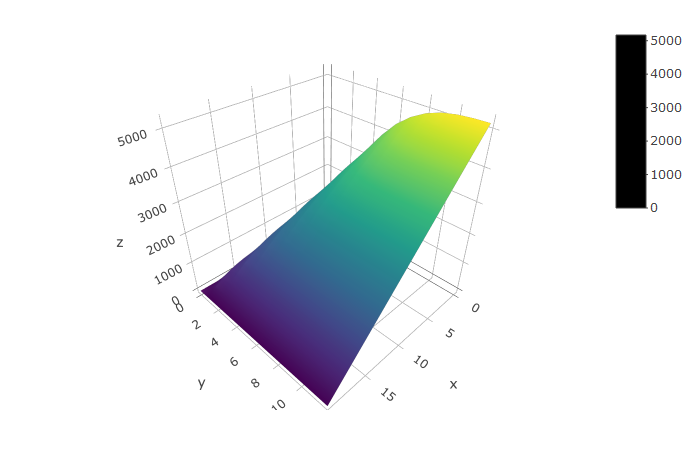
\includegraphics[width=\linewidth]{C:/Users/Stefan/LRZ Sync+Share/Masterarbeit-Klein/Code/Results/smallTest2-False-DP-190619-1333/value_function.png}
\end{figure}

\subsection{Choice based linear programming}

based on Bront et al and van Ryzin.

Taking an eagle-eye perspective, the company has to decide which sets to offer in every single time period, but as the probabilities don't change over time, the specific time point when to offer one set is indistinguishable, we can aggregate over time. Let us introduce a few more notation to get a hand on this. Let $R(\mathbf{x})$ represent the expected revenue given offer set $\boldsymbol{x}$, i.e.

\begin{align}
	R(\boldsymbol{x}) = \sum_{j \in [n]} r_j p_j(x) \quad.
\end{align}

Furthermore, let $\boldsymbol{Q}(\boldsymbol{x}) = (Q_1(\boldsymbol{x}), \dots, Q_m(\boldsymbol{x}))^T$ denote the expected capacity being used, i.e. 

\begin{align}
	Q_h(\boldsymbol{x}) = \sum_{j \in [n]} a_{hj} p_j(\boldsymbol{x}) \quad.
\end{align}

We can denote the total time set $\boldsymbol{x}$ is offered by $t(\boldsymbol{x})$ and the set of all possible offersets as $N = \{0,1\}^n$ . Thus, we can formulate the choice-based linear program (CDLP) \nomenclature{CDLP}{choice-based linear program} as presented in van Ryzin and Liu. Here the optimization problem is solved by varying the decision variables $t(\boldsymbol{x})$.

\begin{align}
	V^{CDLP} = & \max \sum_{\boldsymbol{x}\in N} R(\boldsymbol{x}) t(\boldsymbol{x})\\
	\text{s.t. } & \sum_{\boldsymbol{x}\in N} Q_h(\boldsymbol{x}) t(\boldsymbol{x}) \leq c_h \quad, \forall h\\
	& \sum_{\boldsymbol{x}\in N} t(\boldsymbol{x}) \leq T~,\\
	& t(\boldsymbol{x}) \geq 0 \quad \forall \boldsymbol{x} \in N~.
\end{align}

Korrektheit getestet mit \texttt{C:\textbackslash{}Users\textbackslash{}Stefan\textbackslash{}LRZ Sync+Share\textbackslash{}Masterarbeit-Klein\textbackslash{}Code\textbackslash{}H\_CDLP\_single\_leg.py} - Example0 in settings
Ergebnisse in \texttt{ C:\textbackslash{}Users\textbackslash{}Stefan\textbackslash{}LRZ Sync+Share\textbackslash{}Masterarbeit-Klein\textbackslash{}Code\textbackslash{}Results\textbackslash{}example0-False-CDLPSingleLeg-190621-1808}

\section{Approximate Dynamic Programming}

\subsection{Approximate Policy Iteration}

\begin{algorithm}
	\caption{Approximate policy iteration}\label{alg-API}
	\begin{algorithmic}[1]
		\State Set $\theta_t = 0$ and $\mathbf{\pi}_t = \mathbf{0}$ $\forall t = 1, \dots, T$
		\For{\texttt{k = 1 to K}}
		\State Set $\hat{V}_t = 0$ and $\mathbf{\hat{C}}_t = 0$ $\forall t = 1, \dots, T$
		\For{\texttt{i = 1 to I}}
		\State Set $\hat{r}_t = 0$ and $\mathbf{\hat{c}}_t = 0$ $\forall t = 1, \dots, T$
		\State Initialize $\mathbf{c} = \mathbf{c}^0$
		\For{\texttt{t = 1 to T}}
		\State $\mathbf{\hat{c}}_t \coloneqq \mathbf{c}$
		\State Compute $\mathbf{\pi}(t, \mathbf{c})$ \label{alg-API-calcPi}
		\State Compute $\mathbf{x} = \text{determineOfferset}(\mathbf{\pi}(t, \mathbf{c}), \epsilon_t)$
		\State Simulate a sales event $j' \in \{0, 1, \dots, n\}$
		\If{$j' \in \{ 1, \dots, n\}$}
		\State $\hat{r}_t = r_{j'}$ and $\mathbf{c} = \mathbf{c} - \mathbf{a}_{j'}$
		\EndIf
		\EndFor
		\State Compute $\hat{V}_t^i = \sum_{\tau = t}^{T}\hat{r}_t \quad \forall t = 1, \dots, T$
		\State Assign $\mathbf{\hat{C}}_t^i = \mathbf{\hat{c}}_t \quad \forall t = 1, \dots, T$
		\EndFor
		\State $\left(\theta_t, \pi_t \right) = \text{updateParameters}\left(\hat{V}_t, \mathbf{\hat{C}}_t, \theta_t, \pi_t, k\right) \quad \forall t = 1, \dots, T$ \label{alg-API-updateParam}
		\EndFor
		\Return {$\left(\theta_t, \pi_t \right)  \quad \forall t = 1, \dots, T$}
	\end{algorithmic}
\end{algorithm}

\todoMinor{\Cref{alg-API-updateParam} umschreiben. Weil fuer den update werden alle Parameter auf einmal geupdatet und nicht fuer jeden Zeitschritt separat.}

Overview of parameters:
\begin{enumerate}
	\item $\theta_t$	optimization parameter (offset)
	\item $\mathbf{\pi}_t$	optimization parameter (bid price for each resource)
	\item $\hat{V}_t = 0$	all sample revenues to go for each sample for each time
	\item $\mathbf{\hat{C}}_t = 0$	all sample available capacities for each sample for each resource for each time
	\item $r_t$	sample revenue generated at time $t$
	\item $\mathbf{c}$	available capacities for each resource at current time
	\item $\mathbf{c}^0$	starting capacities
	\item $\mathbf{x}$ offerset at current time
	\item $\epsilon_t$ epsilon used at current time
	
\end{enumerate}

Calculations:

\noindent\rule{\textwidth}{1pt}
$\mathbf{\pi}(t, \mathbf{c}) = \pi_h(t, c_h) \text{ for } h \in [m]$

\begin{numcases}{\pi_h(t, c_h) = }
\infty & if $c_h = 0$ \\
\sum_{s=1}^{S_h} \pi_{ths}\mathbbm{1}_{\left(b_h^{s-1}, b_h^s\right]}(c_h) &  otherwise.
\end{numcases}

\todoRed{Fuer \Cref{alg-API-calcPi} verwende Zeit \textbf{t} statt \textbf{t+1}. Grund: Kenne Informationen zur Zukunft nicht.}

\noindent\rule{\textwidth}{1pt}
The function $\text{determineOfferset}(\mathbf{\pi}, \epsilon)$ calculates the set to offer depending on the current bid prices $\mathbf{\pi}$ via the greedy algorithm layed out in 
%todo add reference
. To account for the exploration vs exploitation dilemma, an epsilon-greedy strategy is used. With a probability of $\epsilon/2$ either no product is offered at all or all products with positive contribution $r_j - \sum_{h \in [m]} a_{hj} \cdot \pi_h$ are offered. With a probability of $1-\epsilon$, the proper calculated set is offered.

\noindent\rule{\textwidth}{1pt}
A sales event is simulated by first having one or zero customer arrive at random. In case a customer arrives, its preference function given the offer set determines the probability according to which one product is sold ($j' \in \{1, \dots, n\}$) or no product is sold ($j' = 0$).

\noindent\rule{\textwidth}{1pt}
%todo Schreibweise der Funktion anpassen, da alle Parameter auf eimal übergeben werden, und nicht separat je Zeitschritt
The function $\left(\theta_t, \pi_t \right) = \text{updateParameters}\left(\hat{V}_t, \mathbf{\hat{C}}_t, \theta_t, \pi_t, k\right)$ really optimizes the following least squares optimization problem for all parameters ($t = 1, \dots, T$) at the same time.

\begin{align}
V_t(\theta_t, \mathbf{\pi}_t, \mathbf{c}_t) & \coloneqq \theta_t + \sum_{h=1}^{m}\sum_{s=1}^{S_h} \pi_{ths} f_{hs}(c_h) \\
f_{hs}(c_h) &\coloneqq 
\begin{cases}\label{def-f}
0 & \text{ if } c_h \leq b_h^{s-1}\\
c_h - b_h^{s-1} & \text{ if } b_h^{s-1} < c_h \leq b_h^s \\
b_h^s - b_h^{s-1} & \text{ if } b_h^s < c_h
\end{cases}
\end{align}

\Cref{def-f} describes the occupied amount of capacity of interval $\left(b_h^{s-1}, b_h^s\right]$.

The following optimization problem depends on the old parameters $\theta_t = \theta_t^k$ and $\mathbf{\pi}_t = \mathbf{\pi}_t^k$ to determine the optimal parameter $\theta_t^{update}$ and $\mathbf{\pi}_t^{update}$.

\begin{alignat}{2}
& \text{min} \sum_{i=1}^{I}\sum_{t=1}^{T} \left( \hat{V}_t^i - V_t(\theta_t, \mathbf{\pi}_t, \mathbf{c}_t^i) \right)^2 && \\
& s.t. && \\
& \theta_t \geq 0 && \forall t\\
& \max_{j=1, \dots, n} r_j \geq \pi_{ths} \geq 0 && \forall t, h, s\\
& \pi_{ths} \geq \pi_{th,s+1} && \forall t, h, s = 1, \dots, S_h-1\\
& \theta_t \geq \theta_{t+1} && \forall t = 1, \dots, T-1\\
& \pi_{ths} \geq \pi_{t+1,hs} && \forall t = 1, \dots, T-1
\end{alignat}

The final parameters $\theta_t^{K+1}$ and $\mathbf{\pi}_t^{K+1}$ can obtained via two possible equally possible ways. One is the so called exponential smoothing, where in each iteration $k$ the parameter for the next iteration $k+1$ is calculated via:
\begin{align}
\theta_t^{k+1} &= \left(1- \frac{1}{k} \right)	\theta_t^k + \frac{1}{k} \theta_t^{update}\\
\mathbf{\pi}_t^{k+1} &= \left(1- \frac{1}{k} \right)	\mathbf{\pi}_t^k + \frac{1}{k} \mathbf{\pi}_t^{update}
\end{align}
The other one uses $\theta_t^{k+1} = \theta_t^{update}$ and $\mathbf{\pi}_t^{k+1} = \mathbf{\pi}_t^{update}$ and averages at the very end.
\begin{align}
\theta_t^{K+1} &= \frac{1}{K}\sum_{k=1}^{K}\theta_t^k\\
\mathbf{\pi}_t^{K+1} &= \frac{1}{K}\sum_{k=1}^{K}\mathbf{\pi}_t^k
\end{align}

\begin{proof}
	\todoMinor{Den Beweis sauber ausfuehren. Hier sind die Inhalte. Die Aussage stimmt, falls die gefundenen optimalen Loesungen in jeder Iteration stets dieselben sind. Dies ist der Fall, wenn es stets nur ein Minimum gibt. Wir haben eine quadratische Zielfunktion, die sozusagen eine mehrdimensionale, nach oben geoeffnete Parabel zeigt, die genau ein globales Minimum besitzt. Weitere noetige Punkte: eindeutiges globales Minimum ueber positiv definite Hesse-Matrix. Optimum auch zulaessig (schwierig?)}
\end{proof}


\subsection{Greedy Heuristic to determine offerset}

The following algorithm is based on the ideas of the greedy heuristic for the column generation subproblem outlined in \cite{Bront.2009}.

Our goal is to determine a reasonable set of products to offer in a fast manner. Thus, we use a heuristic and cut down the amount of products to consider as fast as possible.

\todoRed{Value Funktion gebuendelt dargestellt und ueberall mit $\lambda$. Vergleiche zu Bront et al. 4.2.2, wo in 3. ohne $\lambda$ und in 4.a mit $\lambda$.}

\begin{algorithm}
	\caption{Greedy Heuristic}\label{alg-GreedyHeuristic}
	\begin{algorithmic}[1] % [1] results in line numbers
		% Großes X verwendet, um Menge zu symbolisieren
		\State $\text{Value}(X) \coloneqq \sum_{l=1}^{L} \lambda_l \frac{\sum_{i \in X}(r_i - A_i^T\pi)u_{li}}{\sum_{i \in X}u_{li} + u_{l0}}$
		\State $S\coloneqq \emptyset,\quad S' \coloneqq \left\{j \in N : r_j - A_j^T\pi > 0\right\}$ \label{alg-L1}
		\State $j^* \coloneqq \arg\max_{j \in S'} \text{Value}(\{j\})$
		\Repeat
		\State $S \coloneqq S \cup \{j^*\},\quad S' \coloneqq S'\backslash\{j^*\}$
		\State $j^* \coloneqq \arg \max_{j \in S'} \text{Value}(S \cup \{j\})$
		\Until {$\text{Value}(S \cup \{j^*\}) \leq \text{Value}(S)$\\}
		\Return {$S$}
	\end{algorithmic}
\end{algorithm}

%todo Kommentiere den Algorithmus.
Let $S'$ be the set of products with positive reduced costs, i. \Cref{alg-L1}
%\chapter{Examples}

\section{Example0}

One interesting result is that for exact reproduction of the results of Bront et al for their example0, the empty offerset has to be excluded from the optimization problem. Otherwise (including empty set) results in the same optimal value but via another combination of the decision variables.

\textit{Example 0} represents a small airline network. Three cities are interconnected by three flights (legs), with a capacity vector $\boldsymbol{c} = (10, 5, 5)^T$. The booking horizon consists of $T = 30$ periods and there are five customer segments with preferences as in \Cref{tb-Example0-Customers}

\begin{table}
	\caption{Segment definition for Example 0\label{tb-Example0-Customers}}
	\begin{tabular}{lccccc}
		\toprule
		Segment & $\lambda_l$ & Consideration set & Preference vector & No purchase preference & Description\\
		\midrule
		1 & $0.15$ & $\{1, 5\}$ & $(5, 8)$ & $2$ & Price sensitive, nonstop (A$\rightarrow$C)\\
		\bottomrule
	\end{tabular}
\end{table}

\begin{figure}
	\caption{Airline network for example 0. \label{fig-Example0}}
	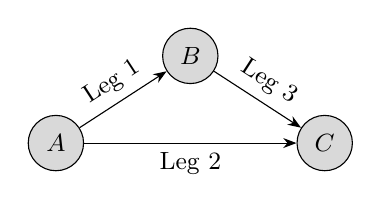
\begin{tikzpicture}[
	mycircle/.style={
		circle,
		draw=black,
		fill=gray,
		fill opacity = 0.3,
		text opacity=1,
		inner sep=0pt,
		minimum size=20pt,
		font=\small},
	myarrow/.style={-Stealth},
	node distance=0.6cm and 1.2cm
	]
	\node[mycircle] (cB) {$B$};
	\node[mycircle,below left=of cB] (cA) {$A$};
	\node[mycircle,below right=of cB] (cC) {$C$};
	
	\foreach \i/\j/\txt/\p in {% start node/end node/text/position
		cA/cB/Leg 1/above,
		cA/cC/Leg 2/below,
		cB/cC/Leg 3/above}
	\draw [myarrow] (\i) -- node[sloped,font=\small,\p] {\txt} (\j);
	
	\end{tikzpicture}
\end{figure}

\begin{table}
	\caption{Airline network for example 0 (products). \label{tb-Example0-Products}}
	\begin{tabular}{yxz}
		\toprule
		\text{Product} & \text{Origin-destination} & \text{Fare}\\
		\midrule
		1 & A \rightarrow C & 1,200\\
		2 & A \rightarrow B \rightarrow C & 800\\
		3 & A \rightarrow B & 500\\
		4 & B \rightarrow C & 500\\
		5 & A \rightarrow C & 800\\
		6 & A \rightarrow B \rightarrow C & 500\\
		7 & A \rightarrow B & 300\\
		8 & B \rightarrow C & 300\\
		\bottomrule
	\end{tabular}
\end{table}
%\chapter{Main chapter}

\section{Ideas}
\begin{enumerate}
	\item capacity consumption $a \in \mathbb{N}_0$ statt $a\in \{0,1\}$
\end{enumerate}

\section{The problem}

Here, we want to lay out the classical revenue management problem an the \enquote{brute force} approach to solve. 

Consider a firm that produces products $j = 1, \dots, n$ with revenues $\boldsymbol{r} = (r_1, \dots, r_n)^T$. Resources $h = 1, \dots, m$ are used for production. In order to produce one unit of product $j$, resources $\boldsymbol{a}_j = (a_{1j}, \dots, a_{mj})^T$ are necessary, with $a_{hj}=1$ if resource $h$ is needed for production of product $j$ and $a_{hj} = 0$ otherwise. Initially, the capacity is described by $\boldsymbol{c}^0 = (c_1^0, \dots, c_m^0)^T$. 

The booking horizon is modelled by sufficiently small time periods $t = 0, \dots, T-1$, such that in each time period at most one customer arrives. This customer also purchases at most one product. If product $j$ is purchased at time $t$, the capacity reduces to $\boldsymbol{c}^{t+1} = \boldsymbol{c}^t - \boldsymbol{a}_j$. Time moves forward, such that the last selling might occur at time $T-1$.

% time index always at the top
The firm wants to increase the value of the products sold and has flexibility in the sets offered. Thus, the decision variables at each time point $t$ are given by $\boldsymbol{x}^t = (x^t_1, \dots, x^t_n)^T$ with $x^t_j = 1$ if product $j$ is offered at time $t$ and $x^t_j = 0$ otherwise.

One popular method of describing the probabilities of purchases is to have each customer belonging to one customer segment $l = 1, \dots L$, each of which following a multinomial logit model (MNL\nomenclature{MNL}{multinomial logit model}). A customer of segment $l$ arrives with probability $\lambda_i$. His preference weights are given by $\boldsymbol{u}_l = (u_{l1}, \dots, u_{ln})^T$ and no purchase preference of $u_{l0}$. Note: $u_{lj} > 0$ if consumer of segment $l$ might purchase product $j$ (the higher, the more interested) and $u_{lj} = 0$ if customer is not interested in product. The probability of purchasing product $j$ when set $\boldsymbol{x}$ is offered is given by $p_{lj}(\boldsymbol{x}) = \frac{u_{lj}x_j}{u_{l0} + \sum_{p\in[n]} u_{lp}x_p}$ and the no-purchase probability is given by $p_{l0}(\boldsymbol{x}) = 1 - \sum_{p\in[n]}p_{lp}$. Together with the uncertainty of which customer segment arrives (if any), we end up at a purchase probability for product $j$ given $\boldsymbol{x}$ of $p_J(\boldsymbol{x}) = \sum_{l \in [L]} p_{lj}(\boldsymbol{x})$.

\subsection{Examples}

\subsubsection{Single-leg flight example}

For reasons of comparability, we use the same example as in \cite{Koch.2017}. An airlines offers four products with revenues $\boldsymbol{r} = (1000, 800, 600, 400)^T$ over $T = 400$ periods. Only one customer segment exists with arrival probability of $\lambda = 0.5$ and preference weights $\boldsymbol{u} = (0.4, 0.8, 1.2, 1.6)^T$. Different network loads can be analyzed by varying initial capacity $c^0 \in \{40, 60, \dots, 120\}$ and varying no-purchase preference weights $u_0 \in \{1,2,3\}$.

\section{Implementation}

Here, we present the results of the exact calculation for the single leg flight example.

Storage folder: \texttt{"C:/Users/Stefan/LRZ Sync+Share/Masterarbeit-Klein/Code/Results/singleLegFlight-True-DP-190611-0917"}

Log:

\verbatiminput{"C:/Users/Stefan/LRZ Sync+Share/Masterarbeit-Klein/Code/Results/singleLegFlight-True-DP-190611-0917/0_logging.txt"}

Results:

\input{"C:/Users/Stefan/LRZ Sync+Share/Masterarbeit-Klein/Code/Results/singleLegFlight-True-DP-190611-0917/erg_paper.txt"}

\section{Approximate Dynamic Programming}

\subsection{Approximate Policy Iteration}

\begin{algorithm}
	\caption{Approximate policy iteration}\label{alg-API}
	\begin{algorithmic}[1]
		\State Set $\theta_t = 0$ and $\mathbf{\pi}_t = \mathbf{0}$ $\forall t = 1, \dots, T$
		\For{\texttt{k = 1 to K}}
		\State Set $\hat{V}_t = 0$ and $\mathbf{\hat{C}}_t = 0$ $\forall t = 1, \dots, T$
		\For{\texttt{i = 1 to I}}
		\State Set $\hat{r}_t = 0$ and $\mathbf{\hat{c}}_t = 0$ $\forall t = 1, \dots, T$
		\State Initialize $\mathbf{c} = \mathbf{c}^0$
		\For{\texttt{t = 1 to T}}
		\State $\mathbf{\hat{c}}_t \coloneqq \mathbf{c}$
		\State Compute $\mathbf{\pi}(t, \mathbf{c})$ \label{alg-API-calcPi}
		\State Compute $\mathbf{x} = \text{determineOfferset}(\mathbf{\pi}(t, \mathbf{c}), \epsilon_t)$
		\State Simulate a sales event $j' \in \{0, 1, \dots, n\}$
		\If{$j' \in \{ 1, \dots, n\}$}
		\State $\hat{r}_t = r_{j'}$ and $\mathbf{c} = \mathbf{c} - \mathbf{a}_{j'}$
		\EndIf
		\EndFor
		\State Compute $\hat{V}_t^i = \sum_{\tau = t}^{T}\hat{r}_t \quad \forall t = 1, \dots, T$
		\State Assign $\mathbf{\hat{C}}_t^i = \mathbf{\hat{c}}_t \quad \forall t = 1, \dots, T$
		\EndFor
		\State $\left(\theta_t, \pi_t \right) = \text{updateParameters}\left(\hat{V}_t, \mathbf{\hat{C}}_t, \theta_t, \pi_t, k\right) \quad \forall t = 1, \dots, T$ \label{alg-API-updateParam}
		\EndFor
		\Return {$\left(\theta_t, \pi_t \right)  \quad \forall t = 1, \dots, T$}
	\end{algorithmic}
\end{algorithm}

\todoMinor{\Cref{alg-API-updateParam} umschreiben. Weil fuer den update werden alle Parameter auf einmal geupdatet und nicht fuer jeden Zeitschritt separat.}

Overview of parameters:
\begin{enumerate}
	\item $\theta_t$	optimization parameter (offset)
	\item $\mathbf{\pi}_t$	optimization parameter (bid price for each resource)
	\item $\hat{V}_t = 0$	all sample revenues to go for each sample for each time
	\item $\mathbf{\hat{C}}_t = 0$	all sample available capacities for each sample for each resource for each time
	\item $r_t$	sample revenue generated at time $t$
	\item $\mathbf{c}$	available capacities for each resource at current time
	\item $\mathbf{c}^0$	starting capacities
	\item $\mathbf{x}$ offerset at current time
	\item $\epsilon_t$ epsilon used at current time
	
\end{enumerate}

Calculations:

\noindent\rule{\textwidth}{1pt}
$\mathbf{\pi}(t, \mathbf{c}) = \pi_h(t, c_h) \text{ for } h \in [m]$

\begin{numcases}{\pi_h(t, c_h) = }
\infty & if $c_h = 0$ \\
\sum_{s=1}^{S_h} \pi_{ths}\mathbbm{1}_{\left(b_h^{s-1}, b_h^s\right]}(c_h) &  otherwise.
\end{numcases}

\todoRed{Fuer \Cref{alg-API-calcPi} verwende Zeit \textbf{t} statt \textbf{t+1}. Grund: Kenne Informationen zur Zukunft nicht.}

\noindent\rule{\textwidth}{1pt}
The function $\text{determineOfferset}(\mathbf{\pi}, \epsilon)$ calculates the set to offer depending on the current bid prices $\mathbf{\pi}$ via the greedy algorithm layed out in 
%todo add reference
. To account for the exploration vs exploitation dilemma, an epsilon-greedy strategy is used. With a probability of $\epsilon/2$ either no product is offered at all or all products with positive contribution $r_j - \sum_{h \in [m]} a_{hj} \cdot \pi_h$ are offered. With a probability of $1-\epsilon$, the proper calculated set is offered.

\noindent\rule{\textwidth}{1pt}
A sales event is simulated by first having one or zero customer arrive at random. In case a customer arrives, its preference function given the offer set determines the probability according to which one product is sold ($j' \in \{1, \dots, n\}$) or no product is sold ($j' = 0$).

\noindent\rule{\textwidth}{1pt}
%todo Schreibweise der Funktion anpassen, da alle Parameter auf eimal übergeben werden, und nicht separat je Zeitschritt
The function $\left(\theta_t, \pi_t \right) = \text{updateParameters}\left(\hat{V}_t, \mathbf{\hat{C}}_t, \theta_t, \pi_t, k\right)$ really optimizes the following least squares optimization problem for all parameters ($t = 1, \dots, T$) at the same time.

\begin{align}
V_t(\theta_t, \mathbf{\pi}_t, \mathbf{c}_t) & \coloneqq \theta_t + \sum_{h=1}^{m}\sum_{s=1}^{S_h} \pi_{ths} f_{hs}(c_h) \\
f_{hs}(c_h) &\coloneqq 
\begin{cases}\label{def-f}
0 & \text{ if } c_h \leq b_h^{s-1}\\
c_h - b_h^{s-1} & \text{ if } b_h^{s-1} < c_h \leq b_h^s \\
b_h^s - b_h^{s-1} & \text{ if } b_h^s < c_h
\end{cases}
\end{align}

\Cref{def-f} describes the occupied amount of capacity of interval $\left(b_h^{s-1}, b_h^s\right]$.

The following optimization problem depends on the old parameters $\theta_t = \theta_t^k$ and $\mathbf{\pi}_t = \mathbf{\pi}_t^k$ to determine the optimal parameter $\theta_t^{update}$ and $\mathbf{\pi}_t^{update}$.

\begin{alignat}{2}
& \text{min} \sum_{i=1}^{I}\sum_{t=1}^{T} \left( \hat{V}_t^i - V_t(\theta_t, \mathbf{\pi}_t, \mathbf{c}_t^i) \right)^2 && \\
& s.t. && \\
& \theta_t \geq 0 && \forall t\\
& \max_{j=1, \dots, n} r_j \geq \pi_{ths} \geq 0 && \forall t, h, s\\
& \pi_{ths} \geq \pi_{th,s+1} && \forall t, h, s = 1, \dots, S_h-1\\
& \theta_t \geq \theta_{t+1} && \forall t = 1, \dots, T-1\\
& \pi_{ths} \geq \pi_{t+1,hs} && \forall t = 1, \dots, T-1
\end{alignat}

The final parameters $\theta_t^{K+1}$ and $\mathbf{\pi}_t^{K+1}$ can obtained via two possible equally possible ways. One is the so called exponential smoothing, where in each iteration $k$ the parameter for the next iteration $k+1$ is calculated via:
\begin{align}
\theta_t^{k+1} &= \left(1- \frac{1}{k} \right)	\theta_t^k + \frac{1}{k} \theta_t^{update}\\
\mathbf{\pi}_t^{k+1} &= \left(1- \frac{1}{k} \right)	\mathbf{\pi}_t^k + \frac{1}{k} \mathbf{\pi}_t^{update}
\end{align}
The other one uses $\theta_t^{k+1} = \theta_t^{update}$ and $\mathbf{\pi}_t^{k+1} = \mathbf{\pi}_t^{update}$ and averages at the very end.
\begin{align}
\theta_t^{K+1} &= \frac{1}{K}\sum_{k=1}^{K}\theta_t^k\\
\mathbf{\pi}_t^{K+1} &= \frac{1}{K}\sum_{k=1}^{K}\mathbf{\pi}_t^k
\end{align}

\begin{proof}
	\todoMinor{Den Beweis sauber ausfuehren. Hier sind die Inhalte. Die Aussage stimmt, falls die gefundenen optimalen Loesungen in jeder Iteration stets dieselben sind. Dies ist der Fall, wenn es stets nur ein Minimum gibt. Wir haben eine quadratische Zielfunktion, die sozusagen eine mehrdimensionale, nach oben geoeffnete Parabel zeigt, die genau ein globales Minimum besitzt. Weitere noetige Punkte: eindeutiges globales Minimum ueber positiv definite Hesse-Matrix. Optimum auch zulaessig (schwierig?)}
\end{proof}


\subsection{Greedy Heuristic to determine offerset}

The following algorithm is based on the ideas of the greedy heuristic for the column generation subproblem outlined in \cite{Bront.2009}.

Our goal is to determine a reasonable set of products to offer in a fast manner. Thus, we use a heuristic and cut down the amount of products to consider as fast as possible.

\todoRed{Value Funktion gebuendelt dargestellt und ueberall mit $\lambda$. Vergleiche zu Bront et al. 4.2.2, wo in 3. ohne $\lambda$ und in 4.a mit $\lambda$.}

\begin{algorithm}
	\caption{Greedy Heuristic}\label{alg-GreedyHeuristic}
	\begin{algorithmic}[1] % [1] results in line numbers
		% Großes X verwendet, um Menge zu symbolisieren
		\State $\text{Value}(X) \coloneqq \sum_{l=1}^{L} \lambda_l \frac{\sum_{i \in X}(r_i - A_i^T\pi)u_{li}}{\sum_{i \in X}u_{li} + u_{l0}}$
		\State $S\coloneqq \emptyset,\quad S' \coloneqq \left\{j \in N : r_j - A_j^T\pi > 0\right\}$ \label{alg-L1}
		\State $j^* \coloneqq \arg\max_{j \in S'} \text{Value}(\{j\})$
		\Repeat
		\State $S \coloneqq S \cup \{j^*\},\quad S' \coloneqq S'\backslash\{j^*\}$
		\State $j^* \coloneqq \arg \max_{j \in S'} \text{Value}(S \cup \{j\})$
		\Until {$\text{Value}(S \cup \{j^*\}) \leq \text{Value}(S)$\\}
		\Return {$S$}
	\end{algorithmic}
\end{algorithm}

%todo Kommentiere den Algorithmus.
Let $S'$ be the set of products with positive reduced costs, i. \Cref{alg-L1}
\chapter{Comparison}

Our goal is to evaluate different policies. One policy is considered better then another policy if it generally leads to higher total revenues. To put this vague phrasing into a scientifically sound comparison, we use an approximate two sample test, which we'll describe here in more detail. We base this overview and notation mainly on Ch. 14.7 of \cite{Bamberg.2011} with extensions as in Ch. 11.3 of \cite{Fahrmeir.2007}.

We have a total of $M$ sample paths each consisting of $T$ time steps, i.e. $M \times T$ random numbers determining which customer arrives and $M \times T$ random numbers leading to which product is purchased. Those two numbers are called \textit{exogenous information}. When applying policy $A$, for each sample path at each time step, the respective offerset is presented to the current customer and its preferences determine which product is purchased. All purchases of one sample path are aggregated and stored, such that policy $A$ results in the vector of values $\mathbf{v}^A \in \mathbb{R}^M$. Accordingly, $\mathbf{v}^B$ is determined. As both policies rely on the same exogenous information, the samples are dependent and a paired samples t-test has to be used.

Thus, we end up with two observations of size $M$ 

$$v^A_1, \dots, v^A_M \text{ respectively } v^B_1, \dots, v^B_M~.$$

%todo notation: A once on top and once on bottom
Let $\bar{\mathbf{v}^A}$ and $S_A^2$ resp. $\bar{\mathbf{v}^B}$ and $S_B^2$ be the empirical mean and empirical variance. Furthermore, $\mu^A$ and $\sigma_A^2$ denote the expected value and variance of $v^A_i$, respectively $\mu^B$ and $\sigma_B^2$ denote the expected value and variance of $v^B_i$. The hypothesis that policy $A$ is better then policy $B$ results in the following null and alternative hypothesis:

$$H_0: \mu^A \leq \mu^B, H_1: \mu^A > \mu^B$$


%\chapter{Thoughts on implementation}

This shall be a short overview of my thoughts regarding the implementation:

\begin{enumerate}
	\item I wanted to produce reproducible results, i.e. my code shall be usable on a larger scope. Logic and Settings shall be separated. Completed code shall be script based and after run, create a folder with its running configuration.
	\item Be careful, when storing list or dataframes, as a deepcopy might have to be used.
	\item 
\end{enumerate}

\chapter{Interesting findings}

\section{DP offer nothing at start}

In the single leg flight scenario with no purchase preference of 1, we found that it makes no difference (due to rounding error), whether just the most expensive product is offered or no product at all. Thus, we want to quickly note this result down here. 

We want to estimate the actions in time $t = 1$. After having the final results computed for all capacities in $t=2$, we arrive at the following values:

\begin{table}
	\begin{tabular}{lrrr}
		\toprule
		{} &    value &  offer\_set\_optimal &  num\_offer\_set\_optimal \\
		\midrule
		0  &      0.0 &                  0 &                      0 \\
		1  &   1000.0 &                  0 &                      2 \\
		2  &   2000.0 &                  0 &                      2 \\
		3  &   3000.0 &                  0 &                      2 \\
		4  &   4000.0 &                  0 &                      2 \\
		5  &   5000.0 &                  0 &                      2 \\
		6  &   6000.0 &                  0 &                      2 \\
		7  &   7000.0 &                  0 &                      2 \\
		8  &   8000.0 &                  0 &                      2 \\
		9  &   9000.0 &                  0 &                      2 \\
		10 &  10000.0 &                  0 &                      2 \\
		11 &  11000.0 &                  0 &                      2 \\
		12 &  12000.0 &                  0 &                      2 \\
		13 &  13000.0 &                  8 &                      1 \\
		14 &  14000.0 &                  8 &                      1 \\
		15 &  15000.0 &                  8 &                      1 \\
		16 &  16000.0 &                  8 &                      1 \\
		17 &  17000.0 &                  8 &                      1 \\
		18 &  18000.0 &                  8 &                      1 \\
		19 &  19000.0 &                  8 &                      1 \\
		20 &  20000.0 &                  8 &                      1 \\
		\bottomrule
	\end{tabular}
	
\end{table}

Furthermore, we have the following offersets:

\begin{table}
	\begin{tabular}{lrrrr}
		\toprule
		{} &  0 &  1 &  2 &  3 \\
		\midrule
		0  &  0 &  0 &  0 &  0 \\
		1  &  0 &  0 &  0 &  1 \\
		2  &  0 &  0 &  1 &  0 \\
		3  &  0 &  0 &  1 &  1 \\
		4  &  0 &  1 &  0 &  0 \\
		5  &  0 &  1 &  0 &  1 \\
		6  &  0 &  1 &  1 &  0 \\
		7  &  0 &  1 &  1 &  1 \\
		8  &  1 &  0 &  0 &  0 \\
		9  &  1 &  0 &  0 &  1 \\
		10 &  1 &  0 &  1 &  0 \\
		11 &  1 &  0 &  1 &  1 \\
		12 &  1 &  1 &  0 &  0 \\
		13 &  1 &  1 &  0 &  1 \\
		14 &  1 &  1 &  1 &  0 \\
		15 &  1 &  1 &  1 &  1 \\
		\bottomrule
	\end{tabular}
	
\end{table}

resulting in the purchase probabilities:

\begin{table}
	\begin{tabular}{lrrrrr}
		\toprule
		{} &         0 &         1 &         2 &         3 &         4 \\
		\midrule
		0  &  0.000000 &  0.000000 &  0.000000 &  0.000000 &  1.000000 \\
		1  &  0.000000 &  0.000000 &  0.000000 &  0.307692 &  0.692308 \\
		2  &  0.000000 &  0.000000 &  0.272727 &  0.000000 &  0.727273 \\
		3  &  0.000000 &  0.000000 &  0.157895 &  0.210526 &  0.631579 \\
		4  &  0.000000 &  0.222222 &  0.000000 &  0.000000 &  0.777778 \\
		5  &  0.000000 &  0.117647 &  0.000000 &  0.235294 &  0.647059 \\
		6  &  0.000000 &  0.133333 &  0.200000 &  0.000000 &  0.666667 \\
		7  &  0.000000 &  0.086957 &  0.130435 &  0.173913 &  0.608696 \\
		8  &  0.142857 &  0.000000 &  0.000000 &  0.000000 &  0.857143 \\
		9  &  0.066667 &  0.000000 &  0.000000 &  0.266667 &  0.666667 \\
		10 &  0.076923 &  0.000000 &  0.230769 &  0.000000 &  0.692308 \\
		11 &  0.047619 &  0.000000 &  0.142857 &  0.190476 &  0.619048 \\
		12 &  0.090909 &  0.181818 &  0.000000 &  0.000000 &  0.727273 \\
		13 &  0.052632 &  0.105263 &  0.000000 &  0.210526 &  0.631579 \\
		14 &  0.058824 &  0.117647 &  0.176471 &  0.000000 &  0.647059 \\
		15 &  0.040000 &  0.080000 &  0.120000 &  0.160000 &  0.600000 \\
		\bottomrule
	\end{tabular}
	
\end{table}

This results in the following expected values, 

$$
[\textbf{1000.}          815.38461538  890.90909091  810.52631579  955.55555556
835.29411765  893.33333333  826.08695652 \textbf{1000.}          840.
907.69230769  828.57142857  963.63636364  852.63157895  905.88235294
840.        ]
$$

i.e. offering nothing and offering just the most expensive product both result in an expected value of $1000$.

As it almost never makes sense to offer no product, we switched the offer set with no products to offer at the very end. The python function \texttt{numpy.amax} returns the index of the first maximum (if there are more than one).



\addcontentsline{toc}{chapter}{Bibliography}
\bibliography{bibliography}
\printnomenclature

\end{document}
